\newpage
\section{Reconocimiento de expresiones matemáticas}

El problema de reconocer expresiones matemáticas en imágenes conciste en encontrar una función capaz de convertir una imagen preprocesada en una secuencia de caracteres que describa en su totalidad la expresión incluida en la imagen. La imagen de entrada $x$ es preprocesada para obtener una imagen en escala de grises de tal forma que $x \in \mathbb{R} ^ {H x W x 1}$, siendo $H$ y $W$ la altura y el ancho de la imagen respectivamente. La secuencia de caracteres objetivo $y$ es de la forma $y_{1}, y_{2}, \dots , y_{k}$ siendo $k$ la longitud de la secuencia y $y_{i}$ es un caracter válido de \LaTeX{} para el presente Trabajo Terminal.

Para resolver el problema de reconocer expresiones matemáticas, existen aproximaciones secuenciales o globales. De acuerdo con \cite{superprecision} ambos métodos implementados de una forma convencional presentan las siguientes limitaciones: 1) La difícil segmentación de símbolos, 2) el análisis estructural es comúnmente basado en gramáticas libres de contexto, lo cual requiere un conocimiento previo de las expresiones a reconocer para diseñar una gramática, 3) la complejidad de los algoritmos de parseo se incrementa con el tamaño de la gramática usada.

Recientemente el modelo de \textit{Encoder-Decoder} con un sistema de atención comenzó a cobrar relevancia por presentar excelentes resultados en campos del machine learning como el procesamiento del lenguaje natural, segmentación de imágenes e \textit{Image Captioning}. Esta aproximación es completamente opuesta a las soluciones convencionales debido a que es una solución entrenable \textit{end-to-end}, es decir, el modelo puede entrenarse como un todo y no por separado; su capacidad de predicción depende completamente del conjunto de entrenamiento por lo que para mejorar el modelo solo se necesita incrementar la cantidad de datos disponibles sin hacer cambios a la arquitectura de la red; la segmentación de símbolos puede hacerse automáticamente a través de la atención. Por las razones expuestas, se decidió utilizar este modelo de deep learning en el presente Trabajo Terminal.

\subsection{Modelo}

Como se mencionó anteriormente la arquitectura de la red neuronal es del tipo \textit{Encoder-Decoder}, en la Figura \ref{fig:modelo} se muestra un esquema de la red neuronal implementada. La traducción de imagenes se realiza de la siguiente manera: Primero se extraen las características de la imágen en forma de grilla utilizando una red convolucional (CNN), luego se procedera a utilizar una versión de dos dimensiones de los \textit{positional encodings} mostrados en el marco teórico y finalmente se procede a reagrupar las filas de la grilla en una sola, esta es la fase de codificación. 

\begin{figure}[H]
    \centering
    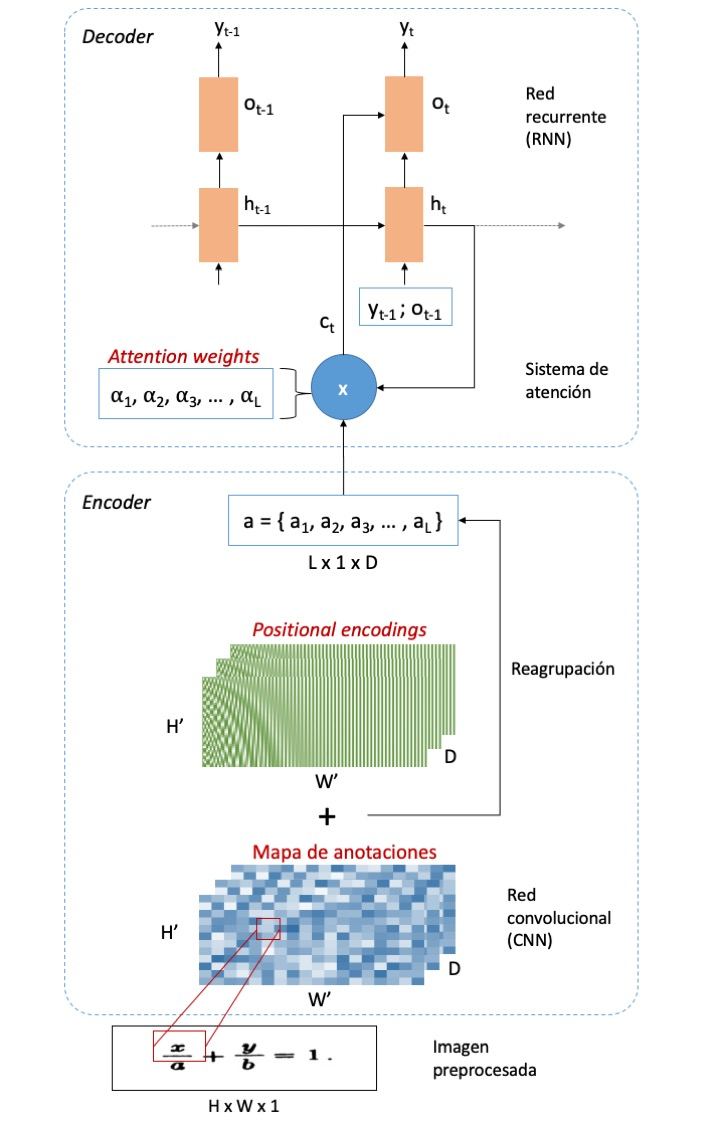
\includegraphics[width=0.8\textwidth]{capitulo5/modelo/img/modelo}
    \caption{Modelo \textit{Encoder-Decoder} de la red neuronal.}
    \label{fig:modelo}
\end{figure}

Para la decodificación, las características codificadas serás usadas por una red neuronal recurrent RNN con un sistema de atención. El \textit{Decoder} implementa un modelo de lenguaje condicional sobre un vocabulario $\lambda$, el cual esta dado por el conjunto de entrenamiento y que será expuesto más adelante.

\subsubsection{Encoder}

La extracción de características de la imagen de entrada $x$ se realiza con una CNN multicapa con \textit{max pooling} y \textit{batch normalization} la cual es ahora un estandar y está completamente inspirada en \cite{harvard}. La Tabla \ref{tbl:cnn-model} sumariza la arquitectura de la red utilizada. Las características extraidas están almacenadas en vector $v \in \mathbb{R} ^ {H' x W' x D}$, siendo $H'$ y $W'$ las nuevas altura y anchura respectivamente y $D$ el tamaño del último filtro de la red, $D = 512$ en este caso.

\begin{table}[]
\centering
\begin{tabular}{@{}|c|c|c|c|c|c|c|c|@{}}
\toprule
\multirow{2}{*}{Número de capa} & \multicolumn{4}{c|}{Capa Convolucional} & \multicolumn{3}{c|}{Capa de Max Pooling} \\ \cmidrule(l){2-8} 
 & \multicolumn{1}{l|}{Kernel} & \multicolumn{1}{l|}{Strides} & \multicolumn{1}{l|}{Padding} & \multicolumn{1}{l|}{BN} & \multicolumn{1}{l|}{Size} & \multicolumn{1}{l|}{Strides} & \multicolumn{1}{l|}{Padding} \\ \midrule
1 & 64-(3,3) & (1,1) & (1,1) & - & (2,2) & (2,2) & (2,2) \\ \midrule
2 & 128-(3,3) & (1,1) & (1,1) & - & (2,2) & (2,2) & (0,0) \\ \midrule
3 & 256-(3,3) & (1,1) & (1,1) & si & \multicolumn{3}{c|}{-} \\ \midrule
4 & 256-(3,3) & (1,1) & (1,1) & - & (2,1) & (2,1) & (0,0) \\ \midrule
5 & 512-(3,3) & (1,1) & (1,1) & si & (1,2) & (1,2) & (0,0) \\ \midrule
6 & 512-(3,3) & (1,1) & (0,0) & si & \multicolumn{3}{c|}{-} \\ \bottomrule
\end{tabular}
\caption{Especificación de la CNN. El 'Kernel' esta denotado como \textit{número de filtros}-(\textit{dimensiones del filtro}).}
\label{tbl:cnn-model}
\end{table}

Se procede a calcular los \textit{positional encodings}. Existen dos formas de hacer esto, la primera es con parámetros aprendidos y la segunda es con valores fijos. El artículo \cite{harvard} utiliza una RNN bidireccional con el vector $v$ como entrada para aprender estos positional encodins. No obstante, acorde con los inventores de esta técnica \cite{attentionisallyouneed}, los positional encodings fijos producen resultados muy similares a los aprendidos. Así, se optó por utilizar positional encodings fijos y se utlizó la generalización a dos dimensiones propuesta por \cite{positionalencodings}. El vector de positional encodings $pe \in \mathbb{R} ^ {H'xW'xD}$ se obtiene con las siguientes ecuaciones:

\begin{equation}
    pe(w,h,2i) = sin\left(\frac{w}{10000 ^ {\frac{4i}{D}}}\right)
\end{equation}

\begin{equation}
    pe(w,h,2i+1) = cos\left(\frac{w}{10000 ^ {\frac{4i}{D}}}\right)
\end{equation}

\begin{equation}
    pe(w,h,2j+D/2) = sin\left(\frac{h}{10000 ^ {\frac{4j}{D}}}\right)
\end{equation}

\begin{equation}
    pe(w,h,2j+1+D/2) = cos\left(\frac{h}{10000 ^ {\frac{4j}{D}}}\right)
\end{equation}

Con esto, se puede obtener el vector de anotaciones $a$ como sigue:

\begin{equation}
    a = v + pe
\end{equation}

Por último, se reagrupa el vector de anotaciones $a$ de tal forma que $a \in \mathbb{R} ^ {LxD}$, donde $L = H' x W'$, así el vector final de salida del \textit{Encoder} es $a = \{ a_{1}, a_{2}, \dots , a_{L} \}$ con $a_{i} \in \mathbb{R} ^ {D}$.

\subsubsection{Decoder}

Las secuencias $y_{t}$ se generan a partir de un modelo de lenguaje condicional que utiliza las anotaciones $a$ obtenidas en el Encoder. La salida del decoder es la probabilidad de obtener el siguiente token dada la historia de tokens previamente generados y el vector de contexto obtenido mediante la atención.

El modelo de lenguaje condicional es como sigue:

\begin{equation}
    p(y_{t}|y_{1}, \dots , y_{t-1}, a) = softmax(W ^ {out}o_{t})
\end{equation}

con

\begin{equation}
    o_{t} = tanh(W ^ {c}[h_{t}; c_{t}])
\end{equation}

\begin{equation}
    h_{t} = LSTM(h_{t-1}, [y'_{t-1}; o_{t-1}])
\end{equation}

\begin{equation}
    y'_{t} = E y_{t-1}
\end{equation}

donde $W ^ {out}$, $W ^ {c}$ y $E$ son parámetros que serán aprendidos. La matríz $E$, es también conocida en la literatura como la matríz de \textit{embeddings}. El vector $h_{t}$ es utilizado para sumarizar toda la historia de decodificación y el vector de contexto $c_{t}$ es usado para capturar la información de contexto de la grilla de características de la imagen $x$. Los corchetes [;], indican una concatenación entre los vectores dentro de ellos.

Para los estados iniciales $h_{0}$ y $o_{0}$ se utilizó un perceptrón multicapa (MLP) que aprendiera los mejores valores iniciales. Las ecuaciones que describen $h_{0}$ y $o_{0}$ respectivamente son:

\begin{equation}
    h_{0} = tanh(W_{h_{0}}a + b_{h_{0}})
\end{equation}

\begin{equation}
    o_{0} = tanh(W_{o_{0}}a + b_{o_{0}})
\end{equation}

En cada instante $t$, el vector de contexto es calculado. Dado que la mayoría de anotaciones $a$ no contienen información útil para decidir el mejor candidato $y_{t}$, el modelo debe de saber cuáles anotaciones atender. Esta tarea, es delegada a un sistema de atención como el propuesto por \cite{bahdanau2014neural}:

\begin{equation}
    e_{t} = u(h_{t}, a)
\end{equation}

\begin{equation}
    \alpha_{t} = softmax(e_{t})
\end{equation}

\begin{equation}
    c_{t} = \phi(\alpha_{t}, a)
\end{equation}

$\phi$ y $u$ son funciones que pueden ser escogidas libremente, en este caso se utilzarón las mismas que en \cite{harvard}:

\begin{equation}
    e_{it} = \beta ^ {T} tanh(W_{h}h_{i-1} + W_{v}a)
    \label{eq:e-attention}
\end{equation}

\begin{equation}
    c_{t} = \sum_{i} ^ {L} \alpha_{it}a_{i}
\end{equation}

donde $W_{h}$ y $W_{v}$ son parámetros que serán aprendidos. Con esto el modelo de atención puede saber que parte de las anotaciones es importante en el instante $t$. Una consecuencia de esto, es que la segmentación de símbolos es delegada también a este sistema.

Finalmente, se decidio modificar la atención para implementar la técnica del \textit{Coverage Vector} como en \cite{chino}. El coverage vector $F$ se incorporó para dar más información al sistema de atención sobre el historial de la misma atentción, de este modo, es posible mejorar la cobertura global del sistema lo cual ayuda a reducir los errores de símbolos no parseados. El vector de coverage se calcula como sigue:

\begin{equation}
    \eta_{t} = \sum_{l}^{t-1} \alpha_{l}
\end{equation}

\begin{equation}
    F = Q * \eta_{t}
    \label{eq:coverage-vector}
\end{equation}

Donde $\eta_{t}$ es la suma de todos los pesos de las attenciones pasadas y $Q$ es una matriz de pesos que serán aprendidos. De este modo, la Ecuación \ref{eq:e-attention} se modifica por:

\begin{equation}
    e_{it} = \beta ^ {T} tanh(W_{h}h_{i-1} + W_{v}a + W_{f}F)
\end{equation}

de donde $W_{f}$ es una matriz de pesos que serán aprendidos.

\subsubsection{Implementación}

El lenguaje de programación utilizado para desarrollar la red fue Python 3 junto con el framework para deep learning TensorFlow 2. Las unidades usadas en el estado $h_{t}$ de la LSTM son $512$ y $80$ para la dimensión de \textit{embedding} para los tokens $80$. El algoritmo de optimización utilizado fue Adam con la Crosentropia Categórica como función de perdida. 

El código que implementa la red es el siguiente:

\lstinputlisting[language=Python]{capitulo5/modelo/src/encoder.py}

\lstinputlisting[language=Python]{capitulo5/modelo/src/decoder.py}

\subsubsection{Entrenamiento}

La red fue entranada en el entorno Colaboratory de Google utilizando una GPU, el proceso de entrenamiento es de alrededor de 30 horas.

Gracias al uso del framework Tensorflow 2, el entrenamiento de la red se puede simplificar mucho. El cálculo de los gradientes de la función de perdida se puede automatizar así como la actualización de los pesos, no obstante, dada la arquitectura de la red, no es posible utilizar los métodos \textit{compile} y \textit{fit} implementados en Keras para Tensorflow 2. Por lo tanto, el ciclo de entrenamiento tuvo que ser diseñado acorde con las necesidades de la arquitectura propuesta.

El código del ciclo de entrenamiento es el siguiente:

\lstinputlisting[language=Python]{capitulo5/modelo/src/training.py}

\subsubsection{Resultados}

\subsubsection{Experimentos Previos}

Antes de encontrar la configuración adecuada para la red neuronal, se llevaron a cabo varios experimentos. A continuación, se presentan los más relevantes.

\vspace{1em}
\textbf{Variante con GRU}
\vspace{1em}

Se utilizó una GRU como en \cite{gru} en lugar de una LSTM en el \textit{Decoder}. No existe un consenso respecto a cual tipo de RNN basadas en compuertas es mejor, por lo que lo más recomendable es experimentar con ambas. En este caso particular, la GRU no logró abstraer las características del problema. El código fuente del \textit{Decoder} con GRU se muestra a continuación:

\lstinputlisting[language=Python]{capitulo5/modelo/src/gru.py}

Una muestra del resultado del entrenamiento se muestra en la Figura \ref{fig:gru-bad}, en (a) vemos que la función de perdida se estanca, demostrando que no es capaz de modelar el problema en su totalidad mientras que en (b), la atención no mostro aprendizaje alguno.

\begin{figure}[H]
    \centering
    \subfigure[Función de perdida más característica del modelo.]{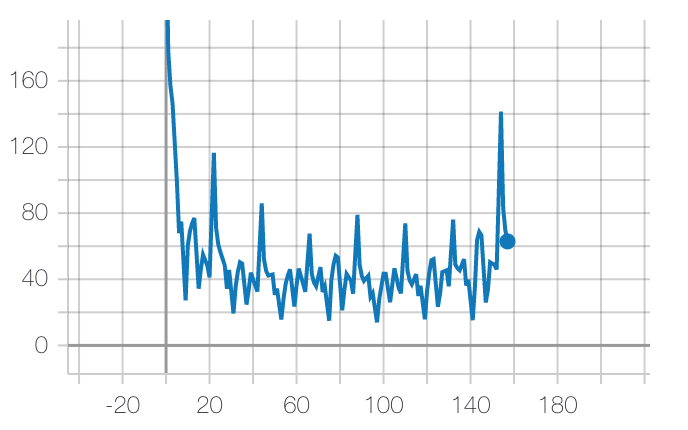
\includegraphics[width=0.5\textwidth]{capitulo5/modelo/img/gru-loss}}
    \subfigure[Atención del sistema.]{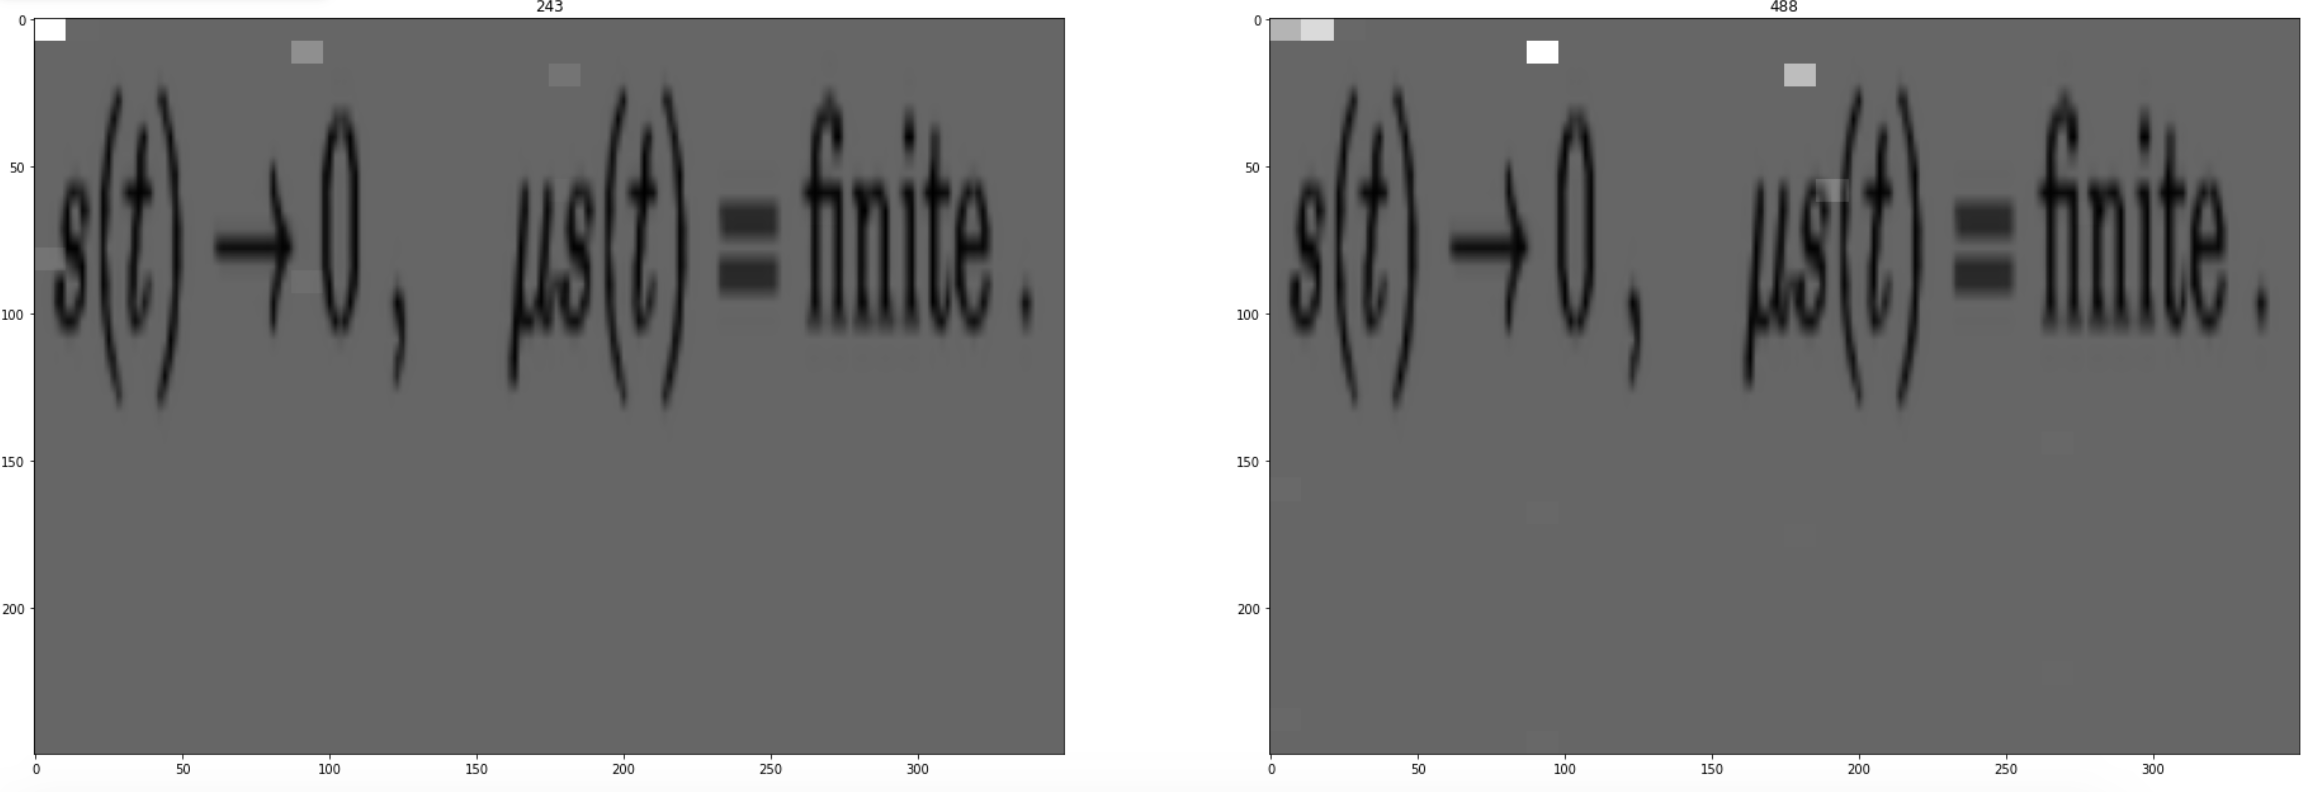
\includegraphics[width=0.5\textwidth]{capitulo5/modelo/img/gru-attention}}
    \caption{(a) Función de perdida del sistema, el modelo se entreno en varias ocasiones, siempre obteniendo una gráfica parecida. (b) Se muestra la atención obtenida por este modelo, se observa un aprendizaje nulo.}
    \label{fig:gru-bad}
\end{figure}


\vspace{1em}
\textbf{Variante con Dropout}
\vspace{1em}

Acorde con \cite{deeplearningbook}, el \textit{dropout} es una técnica utilizada para regularizar redes neuronales, es decir, para que la probabilidad de que un modelo se sobreentrene disminuya. Conciste en aplicar un muestreo a las salidas de alguna capa en un modelo con la finalidad de desactivar un porcentaje de neuronas. Suponiendo a $\mu$ como el vector de muestreo y a $p(\mu)$ como la distribución de probabilidad que modela si la neurona se desactiva o no, podemos aplicar dropout a una capa de alguna red neuronal que modele una distribución $p(y|x)$ de la siguiente manera:

\begin{equation}
    P' = p(\mu)p(y|x,\mu)
\end{equation}

De este modo, algunas neuronas son "desconectadas" haciendo que cada neurona aprenda sobre la información proveida en el entrenamiento de manera independiente. Esto produce también, un efecto de regularización.

La técnica del dropout es recomendada en la mayoría de los modelos de deep learning, sin embargo en el caso del presente Trabajo Terminal no tuvo ningún efecto. Esto es debido posiblemente a que el modelo no es suficientemente profundo para mostrar los efectos del dropout. En la Figura \ref{fig:dropout-bad} se pueden ver los resultados de generales de este modelo.

\lstinputlisting[language=Python]{capitulo5/modelo/src/dropout.py}

\begin{figure}[H]
    \centering
    \subfigure[Función de perdida más característica del modelo.]{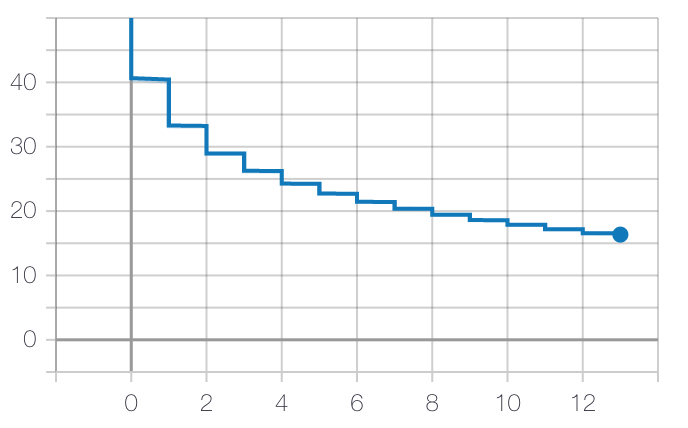
\includegraphics[width=0.5\textwidth]{capitulo5/modelo/img/dropout-loss}}
    \subfigure[Atención del sistema.]{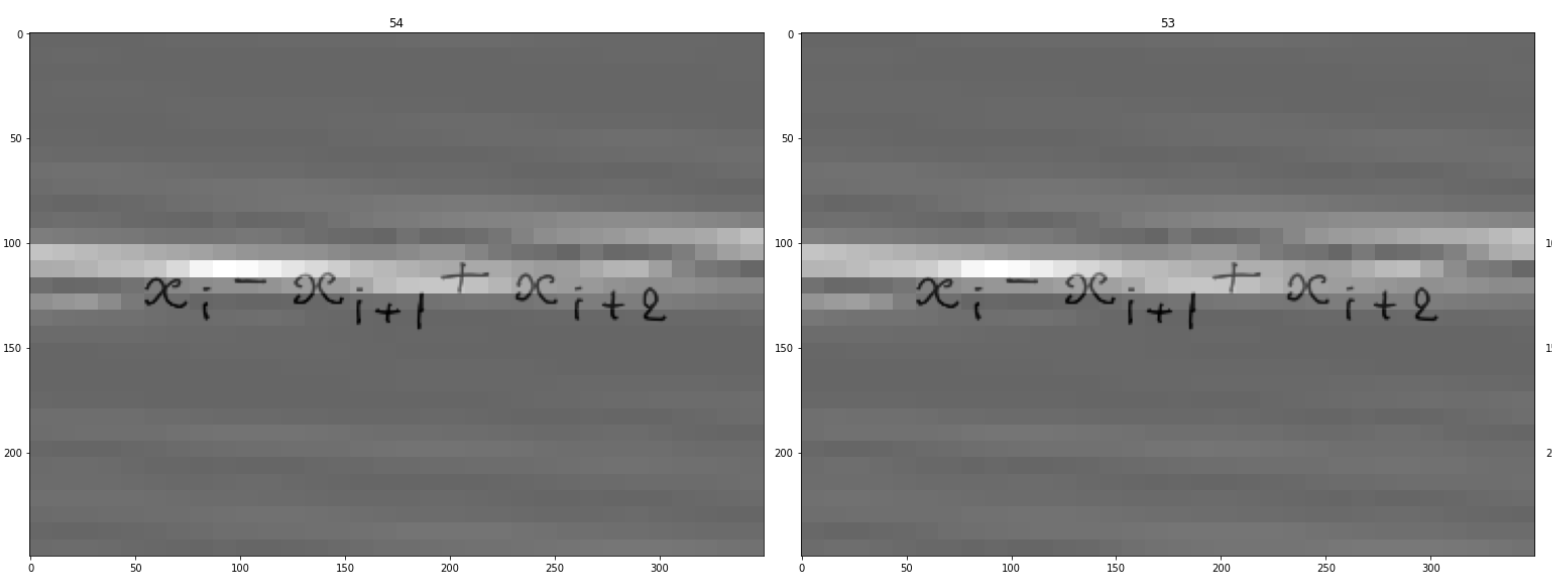
\includegraphics[width=0.5\textwidth]{capitulo5/modelo/img/dropout-attention}}
    \caption{(a) Función de perdida del sistema, el modelo se entreno en varias ocasiones, siempre obteniendo una gráfica parecida. (b) Se muestra la atención obtenida por este modelo, se observa un que el modelo aprendió que a indentificar donde estaba la ecuación, no obstante no aprendio a segmentar los símbolos.}
    \label{fig:dropout-bad}
\end{figure}
 







